\chapter{Related Works}\label{cap:conclusiones}
\noindent The present chapter describes other particular solutions that explore executing MapReduce applications over on-demand infrastructure provisions. Each one's characteristics will be briefly explained and contrasted against qosh's.

\section{Amazon Elastic MapReduce}\label{sec:emc}
\noindent \emph{Amazon Elastic MapReduce} \cite{aws} exposes a web service interface that allows a user to send MapReduce execution requests. EMR is supported internally by Amazon EC2 to provision, on-demand, the infrastructure required by the MapReduce workflow. Thus, an EMR user will not have to worry about provisioning, creating, configuring and destroying the virtual clusters that would support execution. This convenient transparency to the user comes with a series of relatively important limitations:

\begin{description}
    \item[Underlying infrastructure restriction:] Being as it is a service owned by Amazon Inc., it was expected that usage of computational resources out of their reach were limited; and so it is: EMR users will not be able to couple their virtual instances to other clouds that may incur in lower exploitation costs.
    qosh, as it has been shown, separates and exposes responsibilities in a way that using a different cloud, requires only adapting a new Compute module to the particular REST API of the cloud that would be used.
    \item[Installation restriction:] It is not possible to deploy a custom-built VM to execute MapReduce applications in EMR. qosh will handle workflows driving a Hadoop VM with a loose coupling with the deploying subsystem (Fabric) with a doble end:
    \begin{itemize}
        \item To ease VM customizations and upgrades (Kernel, Hadoop, JRE, etc.).
        \item To give the possibility to create custom VMs from scratch.
    \end{itemize}
    \item[Information restriction:] Some users are under non-disclosure agreements that render impossible sharing data with third parties like Amazon, effectively leaving those services out of the equation. qosh's open source nature makes it easy for a developer to adapt qosh to its particular functional requirements with no sharing of private data.
\end{description}

EMR node typology is described next. EMR clusters present three kinds of nodes:

\begin{description}
    \item[Master:] this node, unique per EMR cluster, executes both a NameNode and a JobTracker.
    \item[Core:] This kind of nodes store data and process job tasks. They are basically comprised of a DataNode and a TaskTracker.
    \item[Task:] they only run TaskTracker processes.
\end{description}

qosh deploys clusters with a single hybrid master-worker node --- with NameNode, JobTracker, DataNode and TaskTracker --- being the rest worker nodes --- with DataNode and TaskTracker only. This deployment configuration could be easily altered to fit into diverse use cases by rewriting the \texttt{mapred.fabric.fabfile} module.

Regarding the execution flow, EMR allows for keeping the instances alive when they had finished their scheduled processing to avoid the computational overhead of their spawning. qosh's default behavior is to destroy instances upon completion of each workflow. As expected, defaults may be easily overridden.

EMR draws on Amazon S3 to store input data to Hadoop as well as to write final results. Intermediate information is stored within the virtual instances and is destroyed as they are. qosh uses the file system of the Controller Node to store I/O data from the virtual cluster, and, like EMR, employs the virtual instances' file system to save intermediate data. qosh may also be plugged a different repository to store final results. To that end, a new back-end module would have to be written for Django to correctly locate data and update the DB to point elsewhere.

\section{Resilin}\label{sec:resilin}
\noindent \emph{Resilin}'s \cite{resilin} main intention is to improve EMR by trying to overcome its limitations. The development team has written an API (see figure \ref{fig:arquitecturaresilin}) capable of receiving EMR-like requests that will translate into two kinds of actions:

\begin{itemize}
    \item An interaction flow with an IaaS Cloud to create and destroy instances (what qosh does in its Compute module).
    \item An SSH connection to the virtual Hadoop cluster to configure and execute tasks (what qosh does with its Fabric module).
\end{itemize}

\begin{figure}[tbp]
\begin{center}
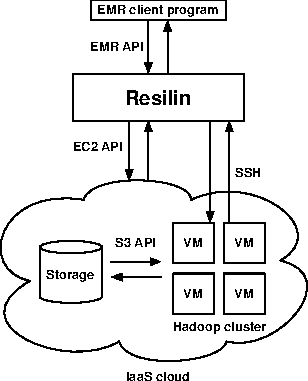
\includegraphics[width=0.5\textwidth]{imagenes/035.pdf}
 \caption{Resilin architecture. Source: \cite{resilin}}
\label{fig:arquitecturaresilin}
\end{center}
\end{figure}

Information storage and I/O is delegated upon an S3 compatibility adaptor supported both by Nimbus and Eucalyptus --- with \emph{Cumulus} and \emph{Walrus} respectively.

Besides, and maybe the most interesting Resilin trait, its developers experiment with the possibility to execute MapRecude workflows atop infrastructure provided by different clouds. Though it may not be the general approach to provision private infrastructure to virtual deployments due to the inherent heterogeneity among different IaaS frameworks, it might prove useful when the infrastructure has to be drawn upon from public clouds. In the abstract, the idea has been implemented bridging deployments on different clouds by exposing instances on one cloud to the other cloud Master Node as if they were part of the same virtual cluster. qosh does not support hybrid cloud deployments. Yet, it cloud be implemented without much ado by modifying the Compute module accordingly.

Another salient feature of Resilin's is the capacity to grow or shrink virtual clusters when the processing had already started. New instances will be assigned tasks as soon as they are registered in the Master process. qosh does not support online cluster resizing.

The bottom line is that Resilin is the solution resembling qosh the most; delegating the reduction of MapReduce workflows on Hadoop and the virtual deployments on an IaaS Cloud EC2-compatible --- all of the four implementations evaluated in \ref{sec:frameworksevaluados} are. Lastly, figure \ref{fig:resilinproyecto} lists the different tools that aid supporting the functionality exposed.

\begin{figure}[tbp]
\begin{center}
\begin{tabular}{|c|c|c|}
\hline
& \textbf{Resilin} & \textbf{qosh} \\
\hline
\textbf{Global} & \texttt{Python} & \texttt{Python} \\
\hline
\textbf{HTTP} & \texttt{Twisted} & \texttt{Django} \\
\hline
\textbf{IaaS Cloud interaction} & \texttt{boto} & \texttt{Compute} (custom module) \\
\hline
\textbf{Virtual instances interaction} & \texttt{paramiko} & \texttt{Fabric} \\
\hline
\end{tabular}
\caption{Tool listing}
\label{fig:resilinproyecto}
\end{center}
\end{figure}

\section{Cloud MapReduce}\label{sec:cloudmapred}
\noindent \emph{Cloud MapReduce} approaches the problem of processing MapReduce workflows over \emph{elastic} infrastructure in a different manner. While Resilin tries to orchestrate executions by putting together every component required to carry computations through, Cloud MapReduce is backed by Amazon's EC2 services to implement the MapReduce model \cite{googlemapreduce} \emph{directly} on top of them.

Following there is a list of the most relevant characteristics of Cloud MapReduce.

\begin{description}
    \item[Incremental scalability:] Is the ability to add new nodes to the virtual cluster when job processing had already begun. New instances will fetch the global job state and will be assigned new tasks as they become online.
    \item[Symmetry and Decentralization:] Is the quality by which Cloud MapReduce will deploy virtual clusters with a flat hierarchy. This feature represents the first separation from what it has been discussed hitherto, where at least one node was in charge of scheduling the execution and storage of others. In Cloud MapReduce the nodes in a virtual cluster collaborate independently from each other, choosing to process the task that would best accommodate their capabilities and that it would work best from a global job perspective. This symmetry makes it easier for a cluster to overcome failing nodes as there is no single point of failure.
    \item[Heterogeneity:] Understood with a double component: On the one hand, the possible coexistence of VMs of different computational flavors in the same workflow; on the other, the ability to create instances on multiple clouds. Resilin supports both features, qosh does not out of the box.
\end{description}

Cloud MapReduce stores I/O and intermediate data into S3. Inter-node communication is solved using Amazon queue service (\emph{SQS} or \emph{Simple Queue Service}). Meta-data is saved in \emph{SimpleDB}.

Lastly, figure \ref{fig:arquitecturacloudmapreduce} represents a high level snapshot of Cloud MapReduce. This figure resembles, not coincidentally, figure \ref{fig:exmapreduce} which showed the typical MapReduce execution phases.

\begin{figure}[tbp]
\begin{center}
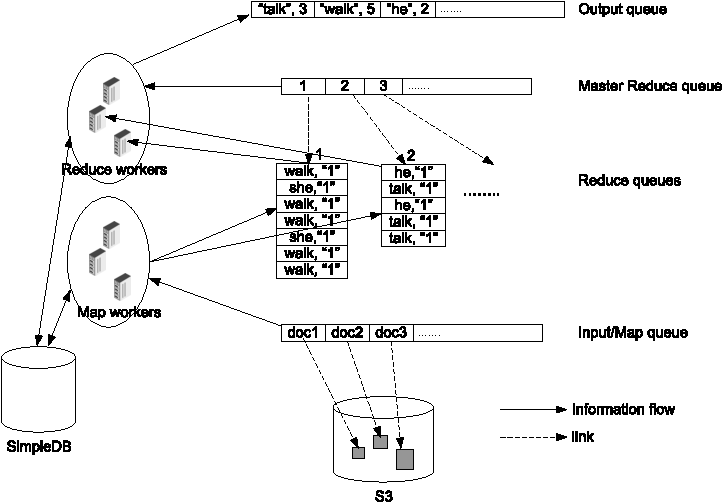
\includegraphics[width=0.9\textwidth]{imagenes/036.pdf}
 \caption{Cloud MapReduce architecture. Source: \cite{cloudmapreduce}}
\label{fig:arquitecturacloudmapreduce}
\end{center}
\end{figure}

\section{Dynamic Cloud MapReduce}\label{sec:dynamicmapreduce}
\noindent Figure \ref{fig:arquitecturadynamicmapreduce} shows the high level architecture of Dynamic Cloud MapReduce \cite{dynamicmapreduce}. It can be easily seen how these high level components directly correspond to qosh's, though Dynamic Cloud MapReduce presents a series of disparities.

\begin{figure}[tbp]
\begin{center}
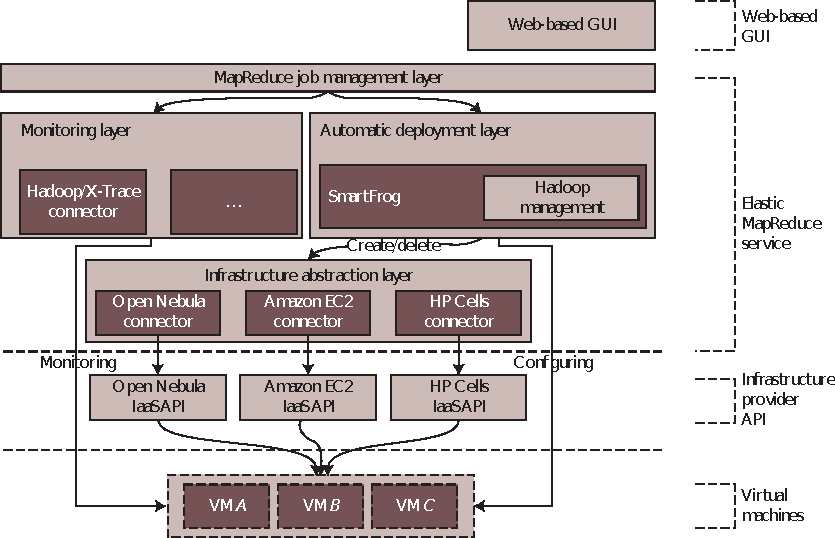
\includegraphics[width=0.9\textwidth]{imagenes/037.pdf}
 \caption{Dynamic Cloud MapReduce. Source: \cite{dynamicmapreduce}}
\label{fig:arquitecturadynamicmapreduce}
\end{center}
\end{figure}

\begin{description}
    \item[GUI:] Dynamic Cloud MapReduce implements a RESTful web service to decouple job management from the particular interface with the user, though the main interaction with the service is through a web site plugged directly to the web service.
    \item[Chain Workflows:] Dynamic Cloud MapReduce allows for chaining MapReduce executions with no need to recreate the virtual cluster to process new jobs.
    \item[Monitoring Layer:] As its name indicates, Dynamic Cloud MapReduce dedicates an independent front-end to oversee the framework status. qosh does not implement a separate layer to supervise the health of the cluster or the evolution of jobs, but this information could be easily extracted from OpenStack Dashboard or Hadoop web interface.
    \item[Automatic Deployment Layer:] Being functionally equivalent to qosh's Fabric module, it controls the virtual deployment. The main difference is that virtual instances are created empty: besides the core OS only \emph{SmartFrog} is installed. Hence, before mapping or reducing, every VM will delegate to SmartFrog the download, installation and configuration of Hadoop.
    While more flexible, this approach introduces an important overhead compared to qosh's preconfigured VM that, nonetheless, would become less significant as the job size increased.
    \item[Infrastructure Provider Abstraction Layer:] This facade separates the REST web service from the particular IaaS Cloud in use, allowing for the definition of adapters to deal with each one. qosh does not abstract an interface to implement different cloud adapters transparently, yet, rewriting the behavior of some functions in the Compute module and accommodating the Transfer Objects to hold the different data would suffice to support any cloud.
\end{description}

Again, the storage back-end is a combination of HDFS and the instances' local file system but it requires the user to manually upload input data to the cluster, instead of managing inputs automatically as qosh does.

\section{Summary}\label{sec:resumenconclusiones}
\noindent Bearing in mind all that has been discussed up to this point, it may be though that qosh is the most limited of the solutions. However, it introduces an important advantage: its utmost simplicity. What could be a subordinate matter comes to the foreground if the user is not an expert or if a quick \emph{elastic} Hadoop test-drive is due.

No other solution presents such a simple and self-contained installation, configuration and infrastructure exploitation. They all need a larger effort from the user to start processing MapReduce workflows. In general, they require: knowing their inner workings, a preexisting deployment of an IaaS cloud, \emph{pay-per-use} or share inputs with third parties. qosh, is the natural choice for initially small deployments or as introductory point to MapReduce and IaaS Cloud technologies. Starting from the minimum automatic deployment, the admin. could add new nodes to the cloud, update the Hadoop VM, alter the infrastructure provisioning mechanics or install another IaaS Cloud with no effort.
